

\documentclass[12pt, letterpaper]{article}

\setlength{\topmargin}{-1.75cm} \setlength{\textheight}{22.5cm}
\setlength{\oddsidemargin}{0.25cm}
\setlength{\evensidemargin}{0.25cm} \setlength{\textwidth}{16.2cm}

% symbols 
\usepackage{fdsymbol}
\usepackage{stmaryrd}
\usepackage{pifont} % check/cross marks 
\newcommand{\cmark}{\ding{51}}%
\newcommand{\xmark}{\ding{55}}%
%\usepackage{amssymb}
\usepackage[ruled,linesnumbered]{algorithm2e}
\usepackage{graphicx}
\usepackage[linguistics]{forest}
% for automata 
\usepackage{tikz} 
\usetikzlibrary{automata,positioning}


\usepackage{palatino, url, multicol} % for multiple columns

\usepackage{pictex}
%% in the .pictex output of xfig, there is command \colo
%% however the old version of pictex may not define this
%% so we define color here as empty
\def \color#1]#2{}

\usepackage{fancyhdr}
\pagestyle{fancy}

\newcommand{\hwnumber} {
    3
}

\newcommand{\hwtitle} {
  Foundation. Languages. Automata.  
}

\newcommand{\duedate}{
    11:59pm Friday October 10}

\date{}

\begin{document}

\newcommand{\hide}[1]{}
\newcommand{\otherquestions}[1]{}
\newcommand{\set}[1]{\{#1\}}
\newcommand{\pg}[1]{{\tt #1}}
\newtheorem{definition}{Definition}
\newcommand{\emptyclause}{\Box}
\newcommand{\keyword}[1]{{\bf #1}}

\newcommand{\ee}[1] {
  \begin{enumerate}
    #1
  \end{enumerate}
}
%% \noindent test \hfill test

\newcommand{\ie}[1] {
  \begin{enumerate}
    #1
  \end{enumerate}
}

\newcommand{\kleene}{\wedge}

\title{{\bf Homework \hwnumber.} \hwtitle}

\maketitle

% Software Verification and Validation was part of collaboration with Professor Namin (see software-vv repository).
\noindent Software Verification and Validation was undertaken in collaboration with Professor Namin. See the software-vv repository for related work.

\vspace{1em}


%\thispagestyle{myheadings} \markright{\courseTitle\ by Y Zhang, TTU,
% \courseDate}

\fancyhf{}
\thispagestyle{fancy}
%
\chead{\courseTitle\ by Y Zhang, TTU,\courseDate}
% \thispagestyle{myheadings} \markright{\courseTitle\ by Y Zhang, TTU,\courseDate}
\cfoot{\thepage}

\noindent {\bf Submit both PDF and latex file of your solution to Canvas by
 \duedate.}

\ee{

  \item  You must use Latex.   
% Use latex to typeset your solution to this homework. You may find the sample latex files here: https://www.overleaf.com/read/czwmmdvqzpcj or the L3-Proof\_twoExamples.tex on blackboard. 

  \item Write pseudo code algorithm: input is a regular expression $R$ and output is the language represented by $R$. (Hint. Study the definition of semantics of regular expression around P59 of L3. Your pseudo code algorithm can be based on problem decomposition/divide and conquer and the definition.) 
  
  Latex sample algorithm:
  
	\begin{algorithm}[H]
		\SetKwInOut{Input}{Input}
		\SetKwInOut{Output}{output}
		\SetKwInOut{SideEffect}{side effect}
		\SetKwInOut{Plan}{plan}
		
		\SetAlgoLined
		\Indm % remove indentation for algorithm "header"
		\Input{ $A[1..n]$: the array of numbers to sort and $n$ is the number of elements in array $A$. }
		\Output{N.A.}
		\SideEffect{The numbers in array $A$ is ordered}
		\Plan{}
		% \SetInd{1em}{1em}
		\Indp
		% all statements in plan is indented 
		\While{While condition}{
			instructions\;
			\eIf{condition}{
				instructions1\;
				instructions2\;
			}{
				instructions3\;
			}
		}
		\caption{sort // this is the name of the algorithm}
	\end{algorithm}
  
  \item Consider the NFA
  \begin{center}
  	
	\begin{tikzpicture}[shorten >=1pt,node distance=2cm,on grid,auto] 
		\node[state,initial] (q_0) at (1.25,2.0)   {$q_0$}; 
		% \node[state] (q_1) [above right=of q_0] {$q_1$}; 
		\node[state](q_1) at (0,0) {$q_1$};
		\node[state, accepting](q_2)  at (2.5,0) {$q_2$};
		\path[->] 
		(q_0) edge  node {a} (q_2)
		(q_0)  edge [above] node {a} (q_1)
		%		          edge  node [swap] {b} (q_1)
		(q_1) edge [below] node {b} (q_2);
	\end{tikzpicture}
   \end{center}
	Write a tuple (as close as the representation used in our definition of NFA) to represent the automaton. 
	% Vice versa.  Similarly for NFA. 
  
  	\item  The {\bf language} accepted by an NFA $N$ is the set of all strings that are accepted by the NFA. Write the definition of this concept using set builder notation.  
  % $\{w | w \mbox{ is accepted by the NFA}\}).
  
	\item Given an automaton below, and a string $0010$, draw the computation tree for $0010$. 
	% Consider the NFA for the language $L = \{ w | w \in \{0, 1\}^* \mbox{ and } w \mbox{ ends with }01\}$. The automata is 
				\begin{center}
		\begin{tikzpicture}[shorten >=1pt,node distance=2cm,on grid,auto] 
			\node[state,initial] (q_0) {$q_0$}; 
			% \node[state] (q_1) [above right=of q_0] {$q_1$}; 
			\node[state](q_1) [right=of q_0] {$q_1$};
			\node[state, accepting](q_2)  [right=of q_1] {$q_2$};
			\path[->] 
			(q_0) edge [loop above] node {$0,1$} ()
			% (q_0) edge  [loop below] node {1} ()
			(q_0) edge  node {$0$} (q_1)
			(q_1) edge  node {$1$} (q_2);
		\end{tikzpicture}
	\end{center}
	
	Latex sample tree (whose content is not related to the answer for this question) below: 
	
  	\begin{center}
		\begin{forest}
			[$q_0$, 
			[$q_1$, edge label={node[midway,left]{a}} 
			[$q_2$, edge label={node[midway,left]{b}}
			[\cmark, edge = dotted]
			]
			]
			[$q_2$, edge label={node[midway,right]{a}}
			[\xmark, edge = dotted]
			]
			]
		\end{forest}
	\end{center}
	
  \item A configuration $(q, w)$ {\bf yields in one step}  configuration $(q', w')$, denoted by $(q, w) \vdash_M (q', w') $ if $w = a w'$ and $\delta(q, a) = q'$.  A configuration $(q_1, w_1)$ {\bf yields}  configuration $(q_2, w_2)$, denoted by $(q_1, w_1) \vdash_M^* (q_2, w_2)$,  if there is a sequence of configurations, starting with $(q_1, w_1)$ and ending with $(q_2, w_2)$, each of which is yielded in one step from its previous configuration. 

  In the definitions above, what are the concepts being defined? concepts used? logical symbols?  important variables? What is the tree structure of the definition statement for {\em yields}? 

  \item Consider an NFA $N = (\Sigma, K, s, F, \Delta)$. Let $M$ be an ``equivalent'' DFA for $N$ as defined in L4. Given $(q_1, aw_1) \vdash_N (q_2, w_1)$ under $N$, prove there exists $S_1, S_2 \in K_M$ such that $(S_1, aw_1) \vdash_M (S_2, w_1)$ under $M$. (Recall our proof methods including application of definition of $\vdash_M$, definition of $\delta$ of $M$, and definitions of DFA and NFAs). 
  % (prove $q_i \in S_i$ in the proof of claim 1)
  
  \item Using the method discussed in class, construct an NFA for  $\llparenthesis a\llparenthesis a \doublecup b \rrparenthesis^\divideontimes \rrparenthesis$. % \doublecup b 
}
\end{document}

